\documentclass{article}
\usepackage{listings}
\usepackage{graphicx}
\usepackage{float}



\begin{document}

\centerline{\sc \large CS 558: Homework 2}
\vspace{.5pc}
\centerline{Alana Laryssa Seabra A Santos}
\centerline{\it 3/14/2016}
\vspace{1pc}

\section{Second problem}

After pre-processing the image using gaussian filter, then using the Hessian detector to extract features and applying non-maximum suppression, I used RANSAC in these point features for detecting lines. My implementation of RANSAC function is able to detect only one line in the given points. In the main code, I called the function 4 times, excluding the inlines for the previous line. Also, I built the version of RANSAC that adaptively determine the number of samples, N is updated for each iteration. \\
For the result below, I used 1px as the distance threshold:

\begin{figure}[ht]
\centering
  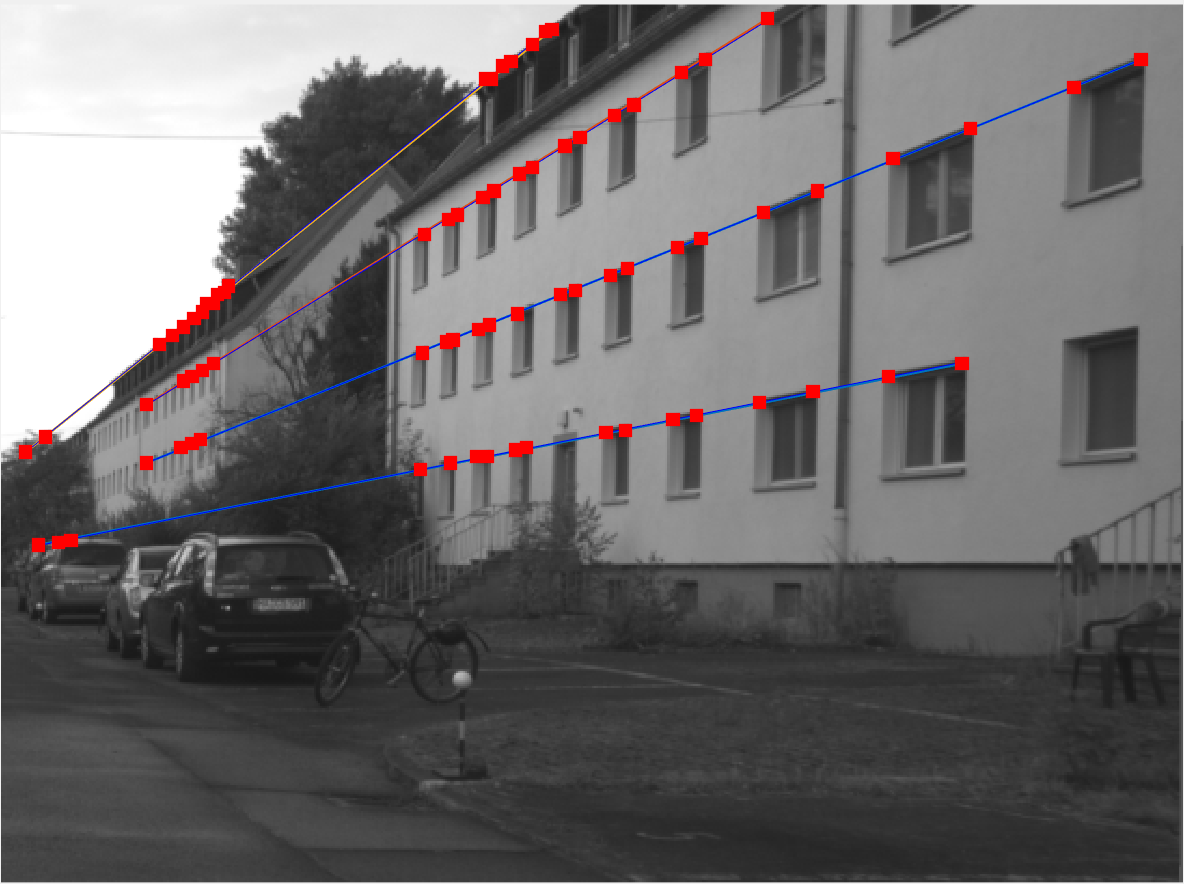
\includegraphics[scale=0.45]{ransac.png}
\end{figure}

\section{Third problem}

My implementation of Hough transform is pretty straightforward. The only detail I guess is worthy mentioning is the limits for $\rho$-space. I used as the limits the norm of the image vector size, so that there's no way that I can calculate a $\rho$ that falls out of bound. \\
Below is the image of the accumulator matrix when using 0.01 as the dimension of the theta bins, in radians, and 1 as the dimension of $\rho$ bins. The intersections pointed in red are the 4 most voted lines. The following image show the lines represented in the original picture.

\begin{figure}[ht]
\centering
  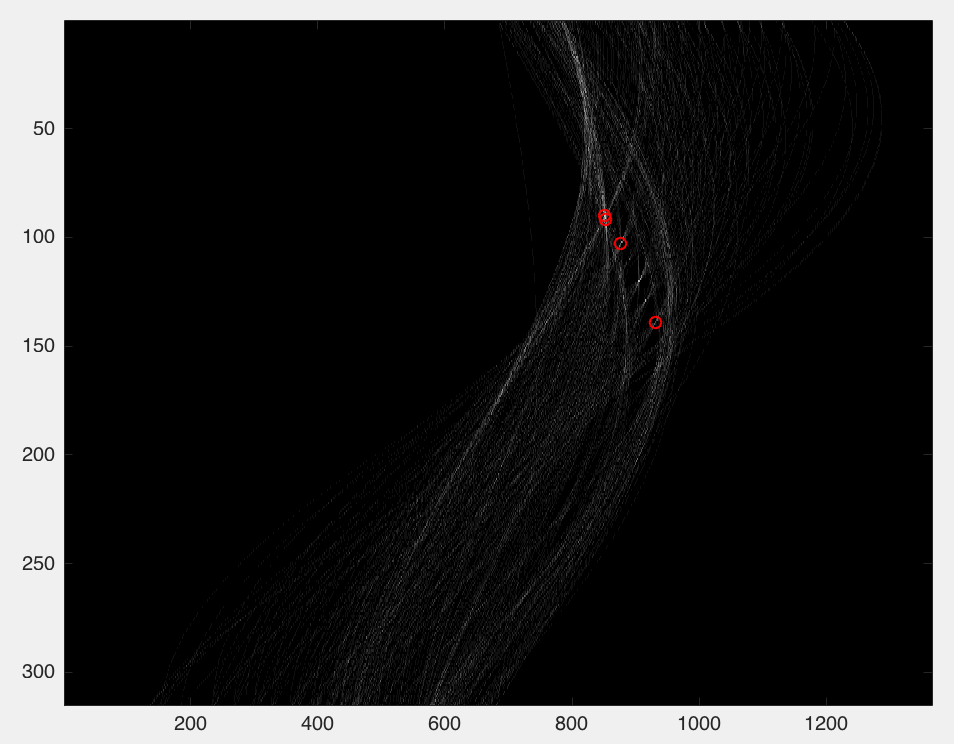
\includegraphics[scale=0.60]{houghspace.png}
\end{figure}


\begin{figure}[h!]
\centering
  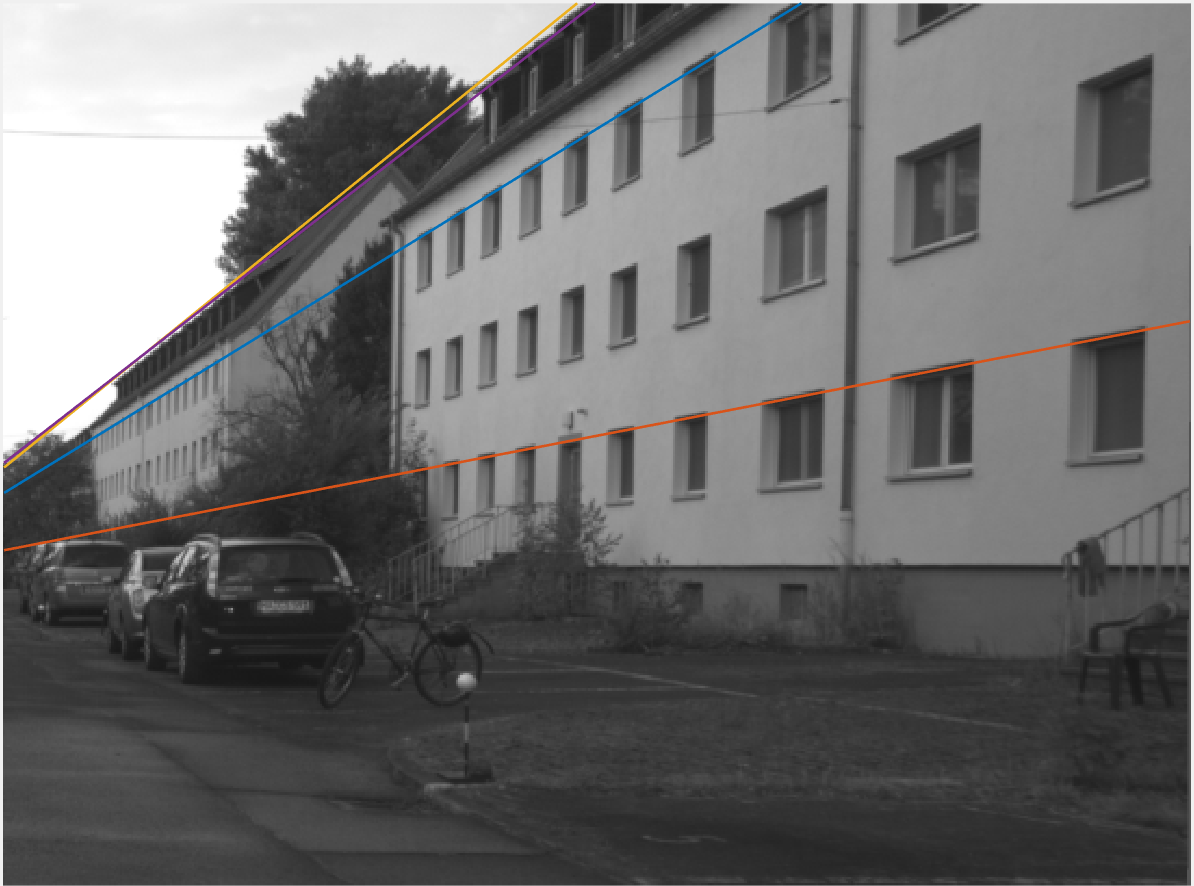
\includegraphics[scale=0.45]{hough.png}
\end{figure}


\section{Matlab code}
\begin{lstlisting}[language=Matlab]

function im2 = filtering (im, f)
 [s1, s2] = size(f);
 hs1 = (s1-1)/2; hs2 = (s2-1)/2;
 im2 = im; 
 for i = hs1+1 : size(im,1) - hs1
     for j = hs2+1 : size(im,2) - hs2
         im2(i,j) = sum(sum(f.*im(i-hs1:i+hs1, j-hs2:j+hs2)));
     end
 end 
end

function im1 = gauss_filter(im,sigma)
    if sigma ~= 0
        halfgauss = 3*sigma - 1;
        [x,y] = meshgrid(-halfgauss:halfgauss, -halfgauss:halfgauss);
        G = exp(-(x.^2 + y.^2)/(2*sigma^2));  % no need to compute the const part
        G = G./sum(G(:));  % sum has to be 1
        im1 = filtering(im, G);
    else
        im1 = im;
    end
end

function im1 = nonmaxsup2(im, half_win) 
    if nargin < 2
        half_win = 1;
    end
    [s1, s2] = size(im);
    im1 = zeros(s1, s2);
    for i = half_win+1:s1-half_win
        for j = half_win+1:s2-half_win
             win = im(i-half_win:i+half_win, j-half_win:j+half_win);
             if max(win(:)) == im(i,j)
                im1(i,j) = im(i,j);
             end
         end
    end   
end


function [bestline, bestinliers] = ransac (pts,t,p,s)

    N = Inf;
    count = 0;
    it = 0;
    bestnuminliers = 0;
    bestline = [];
    bestinliers = [];

    if size(pts,1) == 1
        pts = pts';
    end
    npoints = length(pts);
    
    while N > count      
        % pick 2 points and form a line
        p1 = 0; p2 = 0;
        while(p1 == p2 || p1 == 0 || p2 == 0)
            p1 = round(rand*npoints);
            p2 = round(rand*npoints);
        end
        [a,b,d] = linefrompoints(pts(p1,:), pts(p2,:));
        
        % pick the closests points to the line
        dist = distpointtoline(pts, [a b d]);
        inliers = find(dist <= t);

        if length(inliers) > bestnuminliers
            bestnuminliers = length(inliers);
            bestline = [a b d];
            bestinliers = inliers;
        end
        
        % update parameters
        e = 1 - length(inliers)/length(pts);
        N = log(1-p)/log(1 - power((1-e),s));
        count = count + 1;

        it = it + 1;
    end
    
%     bestinlierspts = pts(bestinliers,:);
%     xx = min(bestinlierspts(:,1)):max(bestinlierspts(:,1));
%     f2 = figure; scatter(pts(:,1),pts(:,2), 'r'), hold on;
%     figure(f2);
%     plot(xx,(bestline(3)-bestline(1).*xx)./bestline(2),'b');
%     scatter(bestinlierspts(:,1),bestinlierspts(:,2),'*','b');
    [it bestnuminliers]
end


function [H,rho,theta] = hough_transform (pts,bintheta,binrho,imagesize)    
    if nargin == 1
        bintheta = 0.01;
        binrho = 1;
        imagesize = [407 548];
    end
    
    if size(pts,1) == 1
        pts = pts';
    end

    npoints = size(pts,1);
    maxrho = norm(imagesize);
    rho = -maxrho:binrho:maxrho;
    theta = 0:bintheta:pi;
    tidx = 1:numel(theta);
    H = zeros(numel(theta), numel(rho));
    
    % filling H
    for i = 1:npoints
        x = pts(i,1); y = pts(i,2);
        r = x.*cos(theta) + y.*sin(theta);
        ridx = round(r + numel(rho)/2);
        idx = sub2ind(size(H),tidx,ridx);
        H(idx) = H(idx) + 1;
    end
end


im = imread('road.png');
im = im2double(im);

% gaussian 
sigma = 1;
im1 = gauss_filter(im,sigma);

% derivatives with sobel filter
Sx = [-1 0 1; -2 0 2; -1 0 1];
Sy = [1 2 1; 0 0 0; -1 -2 -1];
 
im1x = filtering(im1, Sx);
im1y = filtering(im1, Sy);
im1xx = filtering(im1x, Sx);
im1yy = filtering(im1y, Sy);
im1xy = filtering(im1x, Sy);

% hessian
thresh = 2.5;
hessian = im1xx.*im1yy - im1xy.*im1xy;
hessian(hessian < thresh) = 0;

% non maximum suppresion
half_win_hess = 1;
hess = nonmaxsup2(hessian, half_win_hess);

f0 = figure; imshow(hess);

[y,x] = find(hess > 0);

t = 1;  % distance threshold / 1px
s = 2;  % minimum number needed to fit the model
p = 0.95;  % probability at least one sample is free from outliers
numofanswers = 4;

f1 = figure; imshow(im), hold on;

pts = [x y];

% ransac
for answ = 1:numofanswers
    [line, inliersidx] = ransac(pts, t, p, s);
    inliers = pts(inliersidx,:);
    [~,idx1] = min(inliers(:,1));
    [~,idx2] = max(inliers(:,1));
    
    figure(f1);
    plot(inliers([idx1 idx2],1), inliers([idx1 idx2],2), 'LineWidth', 1.2);

    xx = inliers(idx1,1):inliers(idx2,1);
    plot(xx,(line(3)-line(1).*xx)./line(2),'b');
    
    halfwin = 1;
    for i = 1:size(inliers,1)
        px = inliers(i,1); py = inliers(i,2);
        [xx,yy] = meshgrid(px-halfwin:px+halfwin, py-halfwin:py+halfwin);
        hold on;
        sq = scatter(xx(:),yy(:),'filled','square','r');
    end
    
    pts(inliersidx,:) = [];
end

% rough transform
[H,rhos,thetas] = hough_transform([x y],0.01,1,size(im));
f2 = figure;
imagesc(H), colormap('gray'), hold on;
f3 = figure;
imshow(im); hold on;

tempH = H;

for answ = 1:numofanswers
    [maxx,tempidx] = max(tempH(:));
    [ith,irho] = ind2sub(size(H),tempidx);
    
    rho = rhos(irho);
    th = thetas(ith);

    figure(f2); scatter(irho,ith,'r');

    xx = 1:size(im,2);
    yy = (rho - xx.*cos(th))/sin(th);
    figure(f3); plot(xx,yy,'LineWidth',1.3);
    
    tempH(ith,irho) = 0;
end





\end{lstlisting}

\end{document}


